%%% ---------------
%%% PREAMBLE
%%% ---------------
\documentclass[11pt,a4paper]{article}

% Define geometry (without using the geometry package)
\usepackage{geometry}
\geometry{landscape, twocolumn, textwidth=27.8cm, textheight=19.5cm
, columnsep=15mm}

%\frenchspacing						% better looking spacing

% Call packages we'll need
\usepackage[french]{babel}			% french
\usepackage{graphicx}				% images
\usepackage{amssymb,amsmath}		% math
\usepackage{multicol}				% three-column layout
\usepackage{url}					% clickable links
\usepackage{marvosym}				% symbols
\usepackage{wrapfig}				% wrapping text around figures
\usepackage{fontspec}			% font encoding
\usepackage{xunicode}
\usepackage{ragged2e}
\usepackage{titlesec}
\usepackage{framed}
\usepackage{tocvsec2}
% Customize (header and) footer
\usepackage{fancyhdr}
\usepackage{enumitem}
%\pagestyle{fancy}
\pagestyle{empty}
\setmainfont{Carlito}

%\titlespacing\section{0pt}{0pt plus 4pt minus 2pt}{0pt plus 2pt minus 2pt}
%\titlespacing\subsection{0pt}{12pt plus 4pt minus 2pt}{0pt plus 2pt minus 2pt}
%\titlespacing\subsubsection{0pt}{12pt plus 4pt minus 2pt}{0pt plus 2pt minus 2pt}

%\newfontfamily\headingfont[]{Arial}
%\titleformat*{\section}{\Large\bfseries\sffamily}
%\titleformat*{\section}{\Large\headingfont}

%\renewcommand{\headrulewidth}{0.0pt}	% no bar on top of page
%\renewcommand{\footrulewidth}{0.4pt}	% bar on bottom of page

%%% ---------------
%%% DEFINITIONS
%%% ---------------

% Define separators
\newcommand{\HorRule}[1]{\noindent\rule{\linewidth}{#1}} % Creating a horizontal rule
\newcommand{\SepRule}{\noindent							 % Creating a separator
						\begin{center}
							\rule{250pt}{1pt}
						\end{center}
						}						

% Define Title en News input
\newcommand{\JournalName}[1]{%
		\begin{center}	
			%\Huge \usefont{T1}{augie}{m}{n}
            \Large \usefont{T1}{augie}{m}{n}
			#1%
		\end{center}	
		\par \normalsize \normalfont}
		
\newcommand{\JournalIssue}[1]{%
		\hfill \textsc{\mydate \today, No #1}
		\par \normalsize \normalfont}

\newcommand{\NewsItem}[1]{%
\vspace{3pt}
\underline{\textbf{#1}}
	%	%\usefont{T1}{augie}{m}{n} 	
	%	\large \textbf{#1} %\vspace{3pt}
   %     %\Large #1 \vspace{4pt}
	%	%\par 
   %     \normalsize \normalfont
		  }
		
\newcommand{\NewsAuthor}[1]{%
			\hfill by \textsc{#1} \vspace{4pt}
			\par \normalfont}		

%pas de numérotation des sections
\setsecnumdepth{none}
\newlength\defaultparindent
\AtBeginDocument{\setlength\defaultparindent{\parindent}}
%%% ---------------
%%% BEGIN DOCUMENT
%%% ---------------
\begin{document}
\setlength{\parindent}{0pt}
% Title	
% -----




% Other news (1)
% -----
%\vspace{0.5cm}
%	\SepRule
%\vspace{0.5cm}

\begin{center}
\NewsItem{ENTRÉE} \\
SILENCE\\
PRIÈRE D'OUVERTURE
\end{center}

% -----
\NewsItem{PREMIÈRE LECTURE} Is 52, 13 – 53, 12
% -----

\begin{framed}
\NewsItem{PSAUME} 30 (31), 2ab.6, 12, 13-14ad, 15-16, 17.25
%\begin{itemize}
%\item[R/]
%Ô Père, en tes mains
%je remets mon esprit.
%\item[]
%En toi, Seigneur, j’ai mon refuge ;
%garde-moi d’être humilié pour toujours.
%En tes mains je remets mon esprit ;
%tu me rachètes, Seigneur, Dieu de vérité.
%\item[]
%Je suis la risée de mes adversaires
%et même de mes voisins ;
%je fais peur à mes amis,
%s’ils me voient dans la rue, ils me fuient.
%\item[]
%On m’ignore comme un mort oublié,
%comme une chose qu’on jette.
%J’entends les calomnies de la foule :
%ils s’accordent pour m’ôter la vie.
%\item[]
%Moi, je suis sûr de toi, Seigneur,
%je dis : « Tu es mon Dieu ! »
%Mes jours sont dans ta main : délivre-moi
%des mains hostiles qui s’acharnent.
%\item[]
%Sur ton serviteur, que s’illumine ta face ;
%sauve-moi par ton amour.
%Soyez forts, prenez courage,
%vous tous qui espérez le Seigneur !
%\end{itemize}

R/ Ô Père, en tes mains
je remets mon esprit.

\smallskip
En toi, Seigneur, j’ai mon refuge ;
garde-moi d’être humilié pour toujours.
En tes mains je remets mon esprit ;
tu me rachètes, Seigneur, Dieu de vérité.

\smallskip
Je suis la risée de mes adversaires
et même de mes voisins ;
je fais peur à mes amis,
s’ils me voient dans la rue, ils me fuient.

\smallskip
On m’ignore comme un mort oublié,
comme une chose qu’on jette.
J’entends les calomnies de la foule :
ils s’accordent pour m’ôter la vie.

\smallskip
Moi, je suis sûr de toi, Seigneur,
je dis : « Tu es mon Dieu ! »
Mes jours sont dans ta main : délivre-moi
des mains hostiles qui s’acharnent.

\smallskip
Sur ton serviteur, que s’illumine ta face ;
sauve-moi par ton amour.
Soyez forts, prenez courage,
vous tous qui espérez le Seigneur !

\end{framed}

\NewsItem{DEUXIÈME LECTURE} He 4, 14-16 ; 5, 7-9

\NewsItem{ACCLAMATION}
	\begin{itemize}
\item[]
Gloire au Christ parole éternelle du Dieu vivant !
\item[]
Gloire à toi Seigneur !
\end{itemize}


% -----
\begin{framed}
\NewsItem{ÉVANGILE} Passion de notre Seigneur Jésus Christ (Jn 18, 1 – 19, 42)

\texttt{Chant durant la passion}  R. : Mon peuple, que t'ai-je fait ? En quoi
t'ai-je offensé ? Réponds-moi ! Ô Dieu Saint, ô Dieu Saint, fort.
Ô Dieu Saint, ô Dieu Saint, fort, immortel, prends pitié de nous.
\end{framed}
\NewsItem{HOMÉLIE}

\NewsItem{LES GRANDES PRIÈRES}

Christ mort sur la croix, exauce notre prière.

\NewsItem{VÉNÉRATION DE LA CROIX} 
\begin{framed}
O Crux ave, spes unica hoc passionis tempore hoc passionis tempore\\
Auge piis justitiam Reisque dona veniam. Auge piis justitiam\\
Reisque dona veniam. O Crux ave, spes unica hoc passionis tempore hoc
passionis tempore
\end{framed}

\NewsItem{PRÉSENTATION DE LA CROIX} 

\NewsItem{VÉNÉRATION DES FIDÈLES}
\begin{framed}
\begin{itemize}
\item[1.] En ce jour est crucifié Le Créateur du monde,
Il est couronné, Lui, le Roi des cieux. Il est attaché au bois,
L’Époux de l’Église. Nous adorons tes souffrances, Ô Christ notre Dieu.
\item[R.] \textbf{Ô Seigneur, prends pitié de nous, Par ta croix sauve-nous !}
\item[2.] Devant toi, Seigneur Jésus, Tout tremble et se prosterne,
Et que toute langue chante Que tu es Seigneur. Tu acceptes nos souffrances
Pour nous racheter. Tu nous laves par ton sang, Efface nos péchés.
\item[3.] Toi qui, élevé en croix, Détruis tous les enfers. Tu effaces la sentence portée contre tous. Obtiens-nous la pénitence De ton bon larron.
Ô Seigneur, dans ton royaume, De nous souviens toi !
\end{itemize}
\end{framed}

\NewsItem{OFFERTOIRE} Voici l'Homme
\begin{itemize}
\item[R/] : Jésus Christ roi blessé, Dieu couronné de nos épines.
Ô Seigneur prends pitié, que ton pardon nous illumine.
\item[1.] L’homme, voici l’homme, jamais homme n’a parlé comme cet homme.
Roi de silence, roi qui se tait devant l’offense, roi de patience et de beauté.
\item[2.] L’homme, voici l’homme, jamais homme ne fut vrai comme cet homme.
Roi de lumière, roi humilié dans la poussière, roi de prière et de clarté.
\item[3.] L’homme, voici l’homme, jamais homme n’a aimé comme cet homme.
Roi de largesse, roi qui console nos détresses, roi de tendresse en nos duretés.
\end{itemize}

\NewsItem{NOTRE PÈRE}


\begin{framed}
\NewsItem{COMMUNION} Berger du silence

Silence de Dieu, au jardin d’agonie, silence de Dieu qui rend la nuit plus noire.
Silence de Dieu, quand la coupe est à boire, Tu es l’enfantement d’une autre vie où la mort est changée, un matin en victoire.
Dieu, berger du silence...

\smallskip
Silence de Dieu, quand l’Arbre meurt en croix, silence de Dieu, tu deviens
cette sève. Silence de Dieu, qui vit et qui relève, tu donnes le fruit mûr du
Golgotha, qui germe en son tombeau, se redresse et se lève.
Dieu, berger du silence...

\smallskip
Silence de dieu, qui alourdit nos croix, silence de Dieu, au temps de nos
souffrances. Silence de Dieu, qui ressemble à l’absence, tu es saison d’hiver et
de vents froids, où germe en notre sol, lentement, ta Semence.
Dieu, berger du silence...


\end{framed}

\NewsItem{PRIÈRE DE CONCLUSION}

\NewsItem{PRIÈRE DE BÉNÉDICTION}

\NewsItem{CHANT D'ENVOI}
\textbf{R/} : Victoire, tu règneras, ô Croix, tu nous sauveras\\
\textbf{1.} Rayonne sur le monde, qui cherche la vérité.\\
Ô croix source féconde d’amour et de liberté. R/\\
\textbf{2.} Redonne la vaillance au pauvre et au malheureux.\\
C’est toi notre espérance qui nous mènera vers Dieu. R/\\
\textbf{3.} Rassemble tous nos frères à l’ombre de tes grands bras.\\
Par toi, Dieu notre Père au ciel nous accueillera. R/


\NewsItem{SORTIE EN SILENCE}


\NewsItem{Informations paroissiales}

\textit{Les horaires des messes et des célébrations sont affichés à l’extérieur des églises, sur Internet et les réseaux sociaux Facebook et Instagram.}



\begin{framed}
\begin{description}
\item[Célébrations de Pâques]
~\\
Samedi 19 avril              : Vigile Pascale à 20h30 à l’église Sainte-Croix\\
Dimanche 20 avril         : Messe de Pâques à 10h à l’église Saint Jean-Baptiste
\item[Rencontre des confirmands avec Mgr Pascal DELANNOY]
Mardi 22 avril de 18h30 à 20h à l’Archevêché 16 Rue Brûlée, 67000 Strasbourg
\item[Voyage en Côte d’Ivoire du 8 au 17 février 2026]
~\\
Mercredi 23 avril 20h au presbytère : réunion d’information concernant le voyage en Côte d’Ivoire
organisé avec le Diocèse de Grand Bassam à un tarif attractif.
Inscription par mail avant \underline{le 30 avril 2025} à : \texttt{paule.troestler@gmail.com} et/ou   \texttt{nathalie\_dick@yahoo.fr}
\end{description}
\end{framed}


\textbf{Répétitions des chorales}\\
\textbf{Chorales paroissiales} : vendredi 25 avril 20h15 à Sainte Croix\\
\textbf{Groupe \og Dans l’Amour de Dieu \fg} : samedi 26 avril 16h30 à Saint Jean-Baptiste

\begin{multicols}{2}
\textbf{Presbytère Saint Jean-Baptiste}\\
2 rue de l'école 67380 Lingolsheim 03 88 78 16 45\\
\textbf{Permanence :} Vendredi de 10h à 12h et de 17h30 à 19h\\
\textbf{Courriel :} \texttt{danielette67380@gmail.com}\\
\textbf{site internet :} \texttt{stjeanbaptistelingo.fr}\\
\textbf{Instagram :} \texttt{@catho\_lingo}\\
\textbf{Facebook :} \texttt{Catho lingo}\\
\textbf{Permancance Caritas}\\ Vestiaire ouvert le mardi de 14h à 16h\\
\end{multicols}


%         \begin{tabular}{l l l}
%         \multicolumn{3}{c}{\textbf{St Jean-Baptiste}} \\
%  Mardi & 11 fév. & Vêpres 18h15 - 18h30. Pas de messe \\
%Jeudi & 13 fév. & Salut au Saint Sacrement 18h15. Messe 18h30. \\
%    Vendredi & 14 fév. & Laudes 08h45 - 09h00. Pas de messe \\
%        Samedi  & 15 fév. & Messe anticipée 18h00 \\
%    Dimanche & 16 fév. & Pas de messe \\      
%      
%         \multicolumn{3}{c}{\textbf{Ste Croix}} \\
%         Mercredi & 12 fév. & Pas de messe \\ 
%         Dimanche & 16 fév.& Messe 10h30 \\
%    
%        \end{tabular}
  
\newpage

\JournalName{Communauté de Paroisses de Lingolsheim \\
\normalsize \textit{Notre Dame des Sables}
\\ \large \'{E}glise Saint Jean-Baptiste
\\  \normalsize \textit{Vendredi 18 avril 2025}
\\ \large Vendredi Saint}
%\noindent\HorRule{3pt} \\[-0.75\baselineskip]
%\HorRule{1pt}
% -----

% Front article
% -----
%\vspace{0.5cm}
%	\SepRule
%\vspace{0.5cm}

%\begin{center}
\begin{minipage}[h]{1.0\linewidth}
\setlength\parindent{\defaultparindent}
\begin{center}
\og \textit{La Croix : chemin de notre salut} \fg
\end{center}

La passion du Christ est très dramatique. Elle dépasse l’entendement humain. C’est une histoire où se rencontrent la bassesse de l’homme et la grandeur de Dieu. En écoutant cette passion, on ressent un sentiment d’indignation devant l’odieux procès qui conduit à la condamnation d’un innocent. Mais en même temps, on découvre par ailleurs le profond respect et l’immense gratitude envers le Fils de Dieu qui nous a aimé jusqu’au bout, au prix de sa vie.
La croix du Christ, signe d’amour et signe de notre salut. Elle reste pour chacun de nous un mystère.

En ce Vendredi Saint, nous nous réunissons pour méditer sur la Passion-Mort et Résurrection du Christ. Sa vie terrestre n’a pas été longue mais elle a été parfaitement réussie parce qu’elle était centrée sur l’Amour. Elle n’a trouvé sa plénitude qu’au-delà de la mort, dans la résurrection et la communion définitive avec le Père. C’est bien là, le symbole de notre propre aventure personnelle. Et pourtant… nous oublions trop souvent que, sur cette terre, nous ne sommes que des pèlerins. Nous avons trop tendance à nous installer. Nous savons que la Vie Éternelle commence sur terre, mais nous oublions que son terme se situe dans la rencontre définitive de Dieu.
Pour progresser dans l’intelligence du mystère de la croix, il ne suffit pas d’acclamer la croix ou de la vénérer. Ce n’est pas non plus de discuter à perte de vue sur ce mystère. Le plus important c’est de prendre modèle sur le Christ : Il n’a pas attendu le Calvaire pour donner sa vie. Il l’a fait jour après jour au hasard des rencontres, chaque fois qu’il s’est mis au service des petits, des malades et des pauvres.
Beaucoup ont compris que la meilleure manière de porter sa croix c’est de porter celle des autres,
\begin{wrapfigure}{l}{0.1\textwidth}
\vspace{-0.5cm}
\centering
	%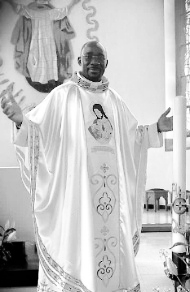
\includegraphics[width=0.1\textwidth]{standing_daniel.png}
	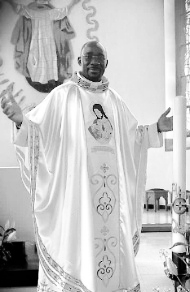
\includegraphics[scale=1.2]{standing_daniel.png}
\end{wrapfigure}
c’est de faire renaître et aider à renaître à l’espérance tous ceux qui sont méprisés, asservis, malades, découragés. C’est ainsi que nous sommes appelés à célébrer la croix du Christ.

En ce Vendredi Saint, les uns pour les autres,
nous prierons
l’Esprit Saint pour qu’il ouvre chacun de nos cœurs à l’intelligence de plus en plus grande de ce mystère d’amour qu’est le mystère de la Croix. Et c’est alors seulement que nous pourrons chanter en toute vérité : \og Victoire ! Tu règneras. Ô croix, tu nous sauveras \fg.



\begin{flushright}
Bonne montée vers Pâques !\\
\textit{Père  Daniel  ETTÉ}
\end{flushright}

\end{minipage}
%\end{center}
% -----
\end{document} 
